\documentclass[aspectratio=169,dvipsnames,usenames]{beamer}
\usepackage{graphicx}
\usepackage{stmaryrd}
\usepackage[T1,T2A]{fontenc}
\usepackage[utf8]{inputenc}
\usepackage[english,russian]{babel}
\usepackage{amsmath}
\usepackage{amsfonts}
\usepackage{amssymb}
\usepackage{makeidx}
\usepackage{verbatim}
\usepackage{amsthm}
%\usepackage{bnf}
\usepackage{tikz}
\usepackage{enumerate}
\usepackage{mathtext}
\usepackage{mathtools}
\usepackage{mathabx}
%\usepackage[left=2cm,right=2cm,top=2cm,bottom=2cm,bindingoffset=0cm]{geometry}
\usepackage{proof}
%\usepackage{paracol}
%\usepackage{enumitem}
\usepackage{xcolor}
\usepackage{colortbl}
%\usepackage{minted}
%\usepackage{hyperref}
\setbeamertemplate{navigation symbols}{}
\usetikzlibrary{graphs}
\usetikzlibrary{graphs.standard}
\usetikzlibrary{automata,positioning}
\usepackage{float}

\begin{document}

%\theoremstyle{dfn}
\newtheorem{dfn}{Определение}[section]
\newtheorem{nte}{Замечание}[section]

\newtheorem{axiom}{Аксиома}[section]
\newtheorem{thm}{Теорема}[section]
\newtheorem{lmm}[theorem]{Лемма}
\newtheorem{statement}{Утверждение}[section]
\newtheorem{oun_paragraph}{Пункт}[section]
\newtheorem{cons}{Следствие}[section]
\newtheorem*{exm}{Пример}

\newcommand{\comb}[1]{\operatorname{\mathcal{#1}}}
\newcommand{\func}[1]{\operatorname{#1}}
\newcommand{\reduction}[1]{{\color{OrangeRed}#1}}
\newcommand{\set}[1]{\left\{#1\right\}}

\def\from#1{\par \parbox{0.7\textwidth}{\par \hfill\raggedleft \it #1}} 

\begin{frame}{}
\begin{center}
{\LARGE Об алгебраической топологии}
\end{center}
\end{frame}

\begin{frame}{Ещё один способ определения эквивалентности}
\begin{thm}$f: A \rightarrow B$, $g : B \rightarrow A$ и $f \circ g = id_B$, $g \circ f = id_A$ тогда и только тогда, когда $f$ биективна и $f^{-1} = g$\end{thm}
\begin{proof}
\begin{itemize}
\item $f$ инъективна, поскольку если найдутся $x_1 \ne x_2: f(x_1) = f(x_2)$, то и $g(f(x_1)) = g(f(x_2))$, значит, $id_A(x_1) = id_A(x_2)$.
\item $f$ сюръективна, поскольку если найдётся $y \in B$, что нет $x : f(x) = y$, то $f(g(y)) \ne y$, т.е. $id_B(y) \ne y$.
\item $f^{-1} = g$, поскольку если $f(x) = y$, то $g(f(x)) = x$.
\end{itemize}

Обратное утверждение очевидно из разбора определения.
\end{proof}
\end{frame}

\begin{frame}{Гомеоморфизм}
\begin{dfn}
Топологические пространства $X$ и $Y$ гомеоморфны ($X \simeq Y$), если найдётся непрерывная биективная $f : X \rightarrow Y$, для которой $f^{-1}$ также непрерывна.
\end{dfn}

\begin{thm}
Гомеоморфизм сохраняет мощность и компактность.
\end{thm}

\begin{exm}
\begin{itemize}
\item Если пространства с дискретной топологией равномощны, то они гомеоморфны (очевидно).
\item $[0,1]$ не гомеоморфен $\mathbb{R}$ (не сохраняется компактность).
\item $(0,1)$ гомеоморфен $\mathbb{R}$: пусть $f(x) = tg(\pi (x - 0.5))$.
\end{itemize}
\end{exm}

\end{frame}

\begin{frame}{Бублик гомеоморфен чашке}
Классическая шутка (файл с Wikimedia Commons, Topology\textunderscore{}joke.jpg, Keenan Crane and Henry Segerman):

\begin{center}
    {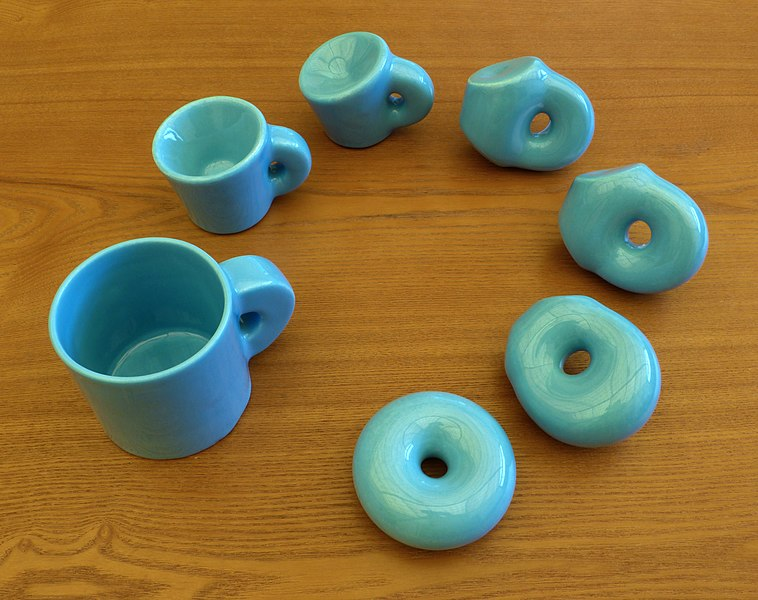
\includegraphics[scale=0.2]{Topology_joke.jpg}}
\end{center}

%Но, конечно, данная картинка доказывает не гомеоморфизм, а гомотопию.
%Однако, доказательство гомеоморфизма использует ещё одну идею: последовательного преобразования.
\end{frame}

\begin{frame}{Гомотопия}
\begin{dfn}
Будем говорить, что непрерывные функции $f_0,f_1: X \rightarrow Y$ гомотопны ($f_0 \sim f_1$), если существует непрерывная функция
$h: X \times [0,1] \rightarrow Y$, что $h(x,0) = f_0$ и $h(x,1) = f_1$. Иначе ещё будем обозначать $h_t(x) := h(x,t)$.
\end{dfn}

%\begin{dfn}
%Петля --- путь $p : I \rightarrow X$, в котором $p(0) = p(1)$.
%\end{dfn}

\begin{exm}
Эти петли гомотопны, $h_t(x) = t (sin 2\pi x, cos 2\pi x)$:

\vspace{-0.3cm}
\begin{center}\tikz{
\draw (0,0) circle [radius=1.6]; \draw (5,0) circle [radius=0.8]; \fill (10,0) circle [radius=0.02];
\draw[-stealth, line width = 0.5] (0,1.6) -- (0.4,1.6); \fill (0,1.6) circle [radius=0.04];
\draw[-stealth, line width = 0.5] (5,0.8) -- (5.4,0.8); \fill (5,0.8) circle [radius=0.04];
\node at (0,-2) { \small $h_1(x) = (\sin 2\pi x, \cos 2\pi x)$ };
\node at (5,-2) { \small $h_{0.5}(x) = \frac{1}{2}(\sin 2\pi x, \cos 2 \pi x)$ };
\node at (10,-2) { \small $h_0(x) = 0(\sin 2\pi x, \cos 2\pi x)$ };
}\end{center}
\end{exm}

\end{frame}

%\begin{thm}
%Гомоптопность является отношением эквивалентности.
%\end{thm}

\begin{frame}{Гомотопическая эквивалентность пространств}
\begin{dfn}
Будем называть топологические пространства $X$ и $Y$ \emph{гомотопически эквивалентными}, если найдутся непрерывные функции
функции $f : X \rightarrow Y$ и $g : Y \rightarrow X$, что $g \circ f \sim id_X$ и $f \circ g \sim id_Y$.
\end{dfn}
\end{frame}

\begin{frame}{$[-1,1] \sim \{0\}$}

$[-1,1] \sim \{0\}$: возьмём $f(x) := 0, g(x) := 0$. Очевидно, что $f(g(y)) \sim id_Y$: возьмём $h^\leftarrow_t(y) = 0$.
В обратную сторону: $h^\rightarrow_t(x) = x\cdot (t)$. Тогда $h^\rightarrow_0(x) = 0 = g(f(x))$, и
$h^\rightarrow_1(x) = x = id_X$

\begin{center}\tikz{

   \node (IA) at (0,-1) { $-1$ };
   \node (IB) at (0,1)  { $1$ };
   \node (P)  at (2,0)  { $0$ };

   \draw (IA) -- (P);
   \draw (IB) -- (P);

   \draw[dashed] (1,-1.5) -- (1,1);
   \draw[-stealth,line width=0.5] (0,-2) -- (2,-2);
}\end{center}\vspace{-0.3cm}

\end{frame}

\begin{frame}{Связности}
\begin{dfn}
Пространство стягиваемо, если оно гомотопически эквивалентно точке (топологическому пространству из одного элемента).
\end{dfn}

\begin{exm}
$S = \{z\in\mathbb{R}^2\ |\ |z| < 1\}$ стягиваемо. Доказательство аналогично написанному выше.
\end{exm}

\begin{dfn}
Пространство линейно связно, если любые две точки соединены путём.

Пространство односвязно, если оно линейно связно и каждая петля в нём гомотопна точке.
\end{dfn}

\end{frame}

\begin{frame}{Сферы}
\begin{dfn}
$S^k := \{ x \in \mathbb{R}^{n+1}\ |\ |x| = 1\}$
\end{dfn}
\begin{exm}
$\mathbb{R}^2\setminus\{\langle 0,0\rangle\} \sim S^1$: пусть $f(\langle x,y \rangle) = \frac{\langle x, y \rangle}{|\langle x, y \rangle|}$, и $g(\langle x,y\rangle) = \langle x, y \rangle$.
\end{exm}
\end{frame}

\begin{frame}{Произведение петель}
\begin{dfn}
Рассмотрим пространство $X$ с отмеченной точкой $x_0 \in X$ и петли $f$ и $g$, что $f(0) = f(1) = g(0) = g(1) = x_0$.
Тогда $$fg (x) = \left\{\begin{array}{ll}f(2x),&x < 0.5\\g(2x-1),&x \ge 0.5\end{array}\right.$$
\end{dfn}
\begin{thm}
Если $f$,$g$,$h$ --- петли в пространстве $\langle X, x_0\rangle$, то \begin{enumerate}
\item $f(gh) \sim (fg)h$
\item Если $e(x) := x_0$, то $fe \sim ef \sim f$
\item Если $f^{-1}(x) := f(1-x)$, то $ff^{-1} \sim f^{-1}f \sim e$.
\end{enumerate}
\end{thm}
\end{frame}

\begin{frame}{Фундаментальная группа}
\begin{dfn}
Группа петель в пространстве $\langle X, x_0\rangle$ --- фундаментальная группа $\pi_1(X,x_0)$.
\end{dfn}

\begin{thm}
Если пространство $X$ линейно-связно, то $\pi_1(X,x_0)$ изоморфна $\pi_1(X,x_1)$ при любом выборе $x_0$ и $x_1$.
\end{thm}
\end{frame}

\begin{frame}{Ветви функции}
\begin{thm}Множество неперерывных отображений $\varphi: S^1 \rightarrow S^1$ и множество непрерывных 
функций $f: [0,1] \rightarrow \mathbb{R}$, что $f(0)=0$ и $f(1) \in \mathbb{Z}$
находятся во взаимно-однозначном соответствии.
\end{thm}

\begin{proof}
Рассмотрим некоторое отображение $\varphi: S^1\rightarrow S^1$ и рассмотрим $\alpha(t) = (sin 2\pi t, cos 2\pi t)$.
Заметим, что уравнение $\alpha(f(x)) = \varphi(\alpha(x))$ позволяет как выразить $f$ по $\varphi$ с точностью
до прибавления целого значения, $\alpha^{-1}(t) \in [0,1)$:
$$f(x) = \alpha^{-1}(\varphi(\alpha(x)))+C_1(x)$$

так и $\varphi$ по $f$: $$\varphi(a) = \alpha(f(\alpha^{-1}(a)))$$

Однако, поскольку $f(0) = 0$ и функция непрерывна, мы можем доопределить $C_1(x)$ единственным образом.
%Заметим, что по непрерывности найдётся такое $n \in \mathbb{N}$, что $\varphi(\alpha(t_1))$ и $\varphi(\alpha(t_2))$
%имеют угловое расстояние меньше $\pi$ при всех $|t_1 - t_2| < \frac{1}{n}$. На каждом из участков 
\end{proof}
\end{frame}

\begin{frame}{Фундаментальная группа $S^1$}
\begin{thm}
Фундаментальная группа $S^1$ эквивалентна группе целых чисел, $\mathbb{Z}$.
\end{thm}
\begin{proof}
Возьмём петлю $\varphi(t) = (sin 2\pi t, cos 2\pi t)$. Тогда $\psi: S^1 \rightarrow S^1$ 
сопоставим петлю $\psi(\varphi(t))$. 

По теореме выше каждому отображению $\psi: S^1 \rightarrow S^1$ можно сопоставить $f_\psi: [0,1] \rightarrow \mathbb{R}$.
Тогда определим отображение группы петель на целые числа так: $|\psi| = f_\psi(1)$. Найдём $|\psi\xi|$:

$$f_{\psi\xi}(x) = 
\left\{
\begin{array}{ll}f_\psi(2x),& x < 0.5
\\ f_\xi(2x-1) + f_\psi(1),& x \ge 0.5
\end{array}
\right.$$
Заметим, что $f_{\psi\xi}$ непрерывна и удовлетворяет граничным условиям, $f_{\psi\xi}(x) = \alpha^{-1}(\psi\xi(\alpha(x))) + C(x)$.
Такая функция единственна, значит, это функция, соответствующая $\psi\xi$. Поэтому $|\psi\xi| = |\psi|+|\xi|$.
Значит, мы задали изоморфизм групп.
\end{proof}
\end{frame}

\begin{frame}{$S^1 \not\sim [0,1]$}
\begin{thm}Если $X \sim Y$, то $\pi_1(X) = \pi_1(Y)$.
\end{thm}

\begin{thm}$S^1 \not\sim [0,1]$\end{thm}
\begin{proof}$\pi_1(S^1) = \mathbb{Z}$, однако $\pi_1([0,1]) = \{0\}$, так как $[0,1]$ стягиваемо.
\end{proof}

\begin{thm}$S^1$ не односвязна.\end{thm}
\end{frame}

\begin{frame}[fragile]{$\pi_1$ в Аренде}
\begin{verbatim}
\instance Aut {A : \1-Type} (a : A) : Group (a = a)
  | ide => idp
  | * => *>
  | ide-left => idp_*>
  | ide-right _ => idp
  | *-assoc => *>-assoc
  | inverse => inv
  | inverse-left => inv_*>
  | inverse-right => *>_inv

\func pi1-1 (X : \1-Type) (x : X) => Aut x

\func pi1Mult {X : \1-Type} {x : X} (a b : pi1-1 X x) => a * b
\end{verbatim}
\end{frame}

\begin{frame}[fragile]{Отображение наматывания}
\begin{verbatim}
\data Sphere1
  | base1
  | loop : base1 = base1
  \where \func ploop => path loop
\end{verbatim}

\begin{verbatim}
\func wind (x : Int) : base1 = base1
  | pos 0 => idp
  | pos (suc n) => wind (pos n) *> path loop
  | neg (suc n) => wind (neg n) *> inv (path loop)
\end{verbatim}

\begin{verbatim}
\func code (x : Sphere1) : \Set0
  | base1 => Int
  | loop i => iso isuc ipred ipred_isuc isuc_ipred i

\func encode (x : Sphere1) (p : base1 = x) : code x => transport code p 0
\end{verbatim}
\end{frame}

\begin{frame}[fragile]{Аксиома унивалентности}
\begin{dfn}
$A \simeq B$, если найдутся $f: A \rightarrow B$, $g: B \rightarrow A$, $f\circ g = id_B$, $g \circ f = id_A$\\
Аксиома унивалентности: $(A \simeq B) \simeq (A = B)$ \end{dfn}

\small
\begin{verbatim}
\func Equiv (A B : \Type) => \Sigma (f : A -> B)
                                    (g : B -> A)
                                    (\Pi (x : A) -> g (f x) = x)
                                    (\Pi (y : B) -> f (g y) = y)
\end{verbatim}
\normalsize

Из равенства легко получить эквивалентность:
\small
\begin{verbatim}
\func equality=>equivalence (A B : \Type) (p : A = B) : Equiv A B =>
  transport (Equiv A) p (\lam x => x, \lam x => x, \lam x => idp, \lam x => idp)
\end{verbatim}
\normalsize

Обратное же постулирует аксиома унивалентности:
\small
\begin{verbatim}
\func equivalence=>equality (A B : \Type) (e : Equiv A B) : A = B =>
  path (iso e.1 e.2 e.3 e.4)
\end{verbatim}
\normalsize
\end{frame}

\begin{frame}[fragile]{Доказательство $\pi_1(S^1) = \mathbb{Z}$}
\begin{verbatim}
\func encode_decode {x : Sphere1} (p : base1 = x) : decode x (encode x p) = p
  | idp => idp

\func encode_wind (x : Int) : encode base1 (wind x) = x
  | ...

\func Loop_S1 : (base1 = base1) = Int =>
  path (iso (encode base1) wind encode_decode encode_wind)
\end{verbatim}

$f : S^1 \rightarrow Int$, $g : Int \rightarrow S^1$, причём $g(f x) = x$ и $f(g x) = x$.
\end{frame}

\end{document}
